\documentclass[11pt,a4paper]{article}
\usepackage[spanish,es-nodecimaldot]{babel}	% Utilizar español
\usepackage[utf8]{inputenc}					% Caracteres UTF-8
\usepackage{graphicx}						% Imagenes
\usepackage[hidelinks]{hyperref}			% Poner enlaces sin marcarlos en rojo
\usepackage{fancyhdr}						% Modificar encabezados y pies de pagina
\usepackage{float}							% Insertar figuras
\usepackage[textwidth=390pt]{geometry}		% Anchura de la pagina
\usepackage[nottoc]{tocbibind}				% Referencias (no incluir num pagina indice en Indice)
\usepackage{enumitem}						% Permitir enumerate con distintos simbolos
\usepackage[T1]{fontenc}					% Usar textsc en sections
\usepackage{amsmath}				% Símbolos matemáticos
\usepackage{listings}
\usepackage{color}

 
\definecolor{codegreen}{rgb}{0,0.6,0}
\definecolor{codegray}{rgb}{0.5,0.5,0.5}
\definecolor{codepurple}{rgb}{0.58,0,0.82}
\definecolor{backcolour}{rgb}{0.95,0.95,0.95}
 
\lstdefinestyle{mystyle}{
    backgroundcolor=\color{backcolour},   
    commentstyle=\color{codegreen},
    keywordstyle=\color{magenta},
    numberstyle=\tiny\color{codegray},
    stringstyle=\color{codepurple},
    basicstyle=\footnotesize,
    breakatwhitespace=false,         
    breaklines=true,                 
    captionpos=b,                    
    keepspaces=true,                 
    numbers=left,                    
    numbersep=5pt,                  
    showspaces=false,                
    showstringspaces=false,
    showtabs=false,                  
    tabsize=2
}
 
\lstset{style=mystyle, language=C++}

% Comando para poner el nombre de la asignatura
\newcommand{\asignatura}{Simulación de Sistemas}
\newcommand{\autor}{José María Sánchez Guerrero}
\newcommand{\titulo}{Práctica 4}
\newcommand{\subtitulo}{Modelos de Simulación Dinámicos Continuos}

% Configuracion de encabezados y pies de pagina
\pagestyle{fancy}
\lhead{\autor{}}
\rhead{\asignatura{}}
\lfoot{Grado en Ingeniería Informática}
\cfoot{}
\rfoot{\thepage}
\renewcommand{\headrulewidth}{0.4pt}		% Linea cabeza de pagina
\renewcommand{\footrulewidth}{0.4pt}		% Linea pie de pagina

\begin{document}
\pagenumbering{gobble}

% Pagina de titulo
\begin{titlepage}

\begin{minipage}{\textwidth}

\centering


\includegraphics[scale=0.5]{img/ugr.png}\\

\textsc{\Large \asignatura{}\\[0.2cm]}
\textsc{GRADO EN INGENIERÍA INFORMÁTICA}\\[1cm]

\noindent\rule[-1ex]{\textwidth}{1pt}\\[1.5ex]
\textsc{{\Huge \titulo\\[0.5ex]}}
\textsc{{\Large \subtitulo\\}}
\noindent\rule[-1ex]{\textwidth}{2pt}\\[3.5ex]

\end{minipage}

\vspace{0.5cm}

\begin{minipage}{\textwidth}

\centering

\textbf{Autor}\\ {\autor{}}\\[2.5ex]
\textbf{Rama}\\ {Computación y Sistemas Inteligentes}\\[2.5ex]
\vspace{0.3cm}


\includegraphics[scale=0.3]{img/etsiit.jpeg}

\vspace{0.7cm}
\textsc{Escuela Técnica Superior de Ingenierías Informática y de Telecomunicación}\\
\vspace{1cm}
\textsc{Curso 2019-2020}
\end{minipage}
\end{titlepage}

\pagenumbering{arabic}
\tableofcontents
\thispagestyle{empty}				% No usar estilo en la pagina de indice

\newpage

\setlength{\parskip}{1em}

\section{Introducción}

En esta práctica nos enfrentamos al modelo de ecosistema de Lotka-Volterra, el cual pretende estudiar el crecimiento entre dos especies
relacionadas entre sí. De estas dos, una de ellas serán los \textbf{depredadores ($x$)} y la otra las \textbf{presas ($y$)}.

Hay varias cosas a tener en cuenta en el modelo. Por ejemplo, en ausencia de presas, la población de depredadores disminuye; mientras que
en ausencia de depredadores, la población de presas aumenta. Tampoco tendremos factores de autoinhibición. Las ecuaciones de crecimiento
de ambas poblaciones se pueden describir de la siguiente forma:
$$\frac{\partial x}{\partial t} = a_{11}x-a_{12}xy$$
$$\frac{\partial y}{\partial t} = a_{21}xy-a_{22}y$$

Los valores de $a_{11}$ y $a_{22}$ representan las tasas de crecimiento de cada una de las especies, y por otro lado, $a_12$ y $a_21$ son los
factores de inhibición mutuos teniendo en cuenta a la otra población.


\section{Programar modelo}
El modelo anterior estará implementado en el archivo \textit{depredadores.cpp} adjuntado con la memoria. El programa partirá del pseudocódigo
proporcionado y además se adaptará a las especificaciones comentadas. Dispondrá de dos métodos de derivación diferentes, uno sencillo utilizando
Euler (aunque no sea recomendable), y otro utilizando el método de Runge-Kuta.

Los parámetros que le podremos pasar al programa será los 4 $a_{ij}$ comentados y los valores iniciales para los depredadores y las presas.
Junto con este programa, también voy a adjuntar un $script$ en python que, utilizando este modelo y los parámetros deseados, nos muestra una
gráfica con la evolución de la población entre el instante inicial y el final.

A continuación, vamos a realizar varias pruebas de nuestro modelo para comprobar su funcionamiento.


\newpage
\section{Experimentación inicial}

Podremos estimar las constantes de las ecuaciones con ayuda de las siguientes suposiciones:
\begin{itemize}
	\item Cada pareja de conejos engendra un promedio de 10 crías por año.
	\item Cada zorro captura un promedio de 25 conejos por año.
	\item La edad promedio de los zorros es de 5 años (20\% de los zorros muere anualmente).
	\item En media, el número medio de zorros jóvenes que sobreviven es igual al número de conejos dividido por 25.
\end{itemize}

Con esto tenemos que los valores iniciales para cada una de las constantes son: $a_{11}=5$, $a_{12}=0.05$, $a_{21}=0.0004$ y $a_{22}=0.2$.
Las poblaciones iniciales para los depredadores y las presas serán las siguientes:
$$depredadores(x) = \frac{a_{11}}{a_{12}} = 100$$
$$presas(y) = \frac{a_{22}}{a_{21}} = 500$$

Utilizaremos el método de integración de Runge-Kuta, junto con un intervalo de cálculo de $h=0.1$. El resultado ha sido el siguiente:
\begin{figure}[H]
\centering
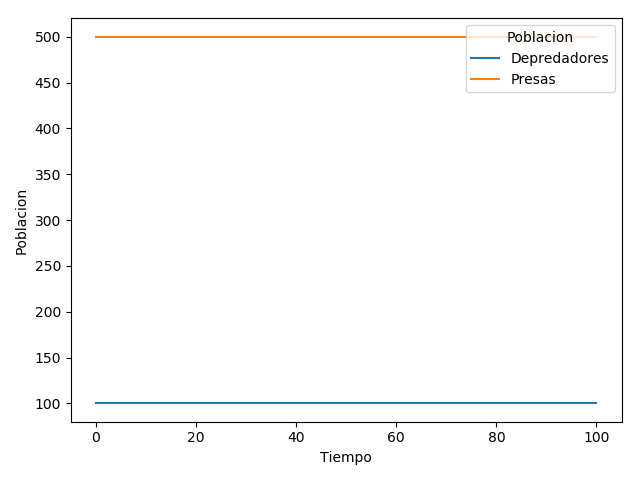
\includegraphics[scale=0.65]{img/2-100-500.png}
\caption{depredadores x->100,   presas y->500}
\end{figure}

Como podemos observar, estos valores mantienen el sistema constante. Hemos conseguido el equilibrio perfecto, ya que ninguno de los niveles
de la población están cambiando, es decir, el resultado de ambas derivadas en igual a 0.

Vamos a distanciar progresivamente los valores de $x$ e $y$ para ver cómo evoluciona la población en esos casos. Probaremos aumentando las
presas en 10, disminuyendo los depredadores en 10, haciendo las dos anteriores juntas, y aumentando en 50 las presas y disminuyendo en 50
los depredadores. Las gráficas resultantes han sido las siguientes:
\begin{figure}[H]
	\centering
	\begin{minipage}{0.5\textwidth}
	  \centering
	  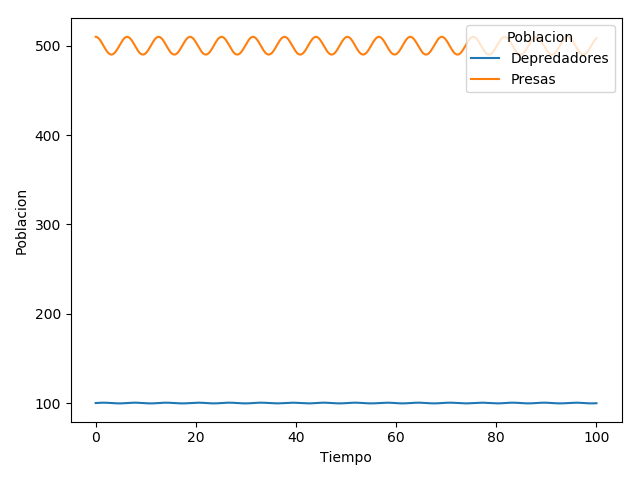
\includegraphics[scale=0.4]{img/2-100-510.png}
	  \caption{x=100,  y=510}
	\end{minipage}%
	\begin{minipage}{0.5\textwidth}
	  \centering
	  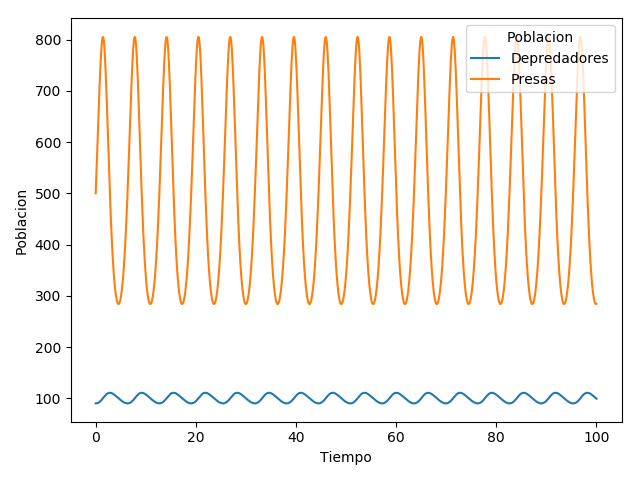
\includegraphics[scale=0.4]{img/2-90-500.png}
	  \caption{x=90,  y=500}
	\end{minipage}
\end{figure}

\begin{figure}[H]
	\centering
	\begin{minipage}{0.5\textwidth}
	  \centering
	  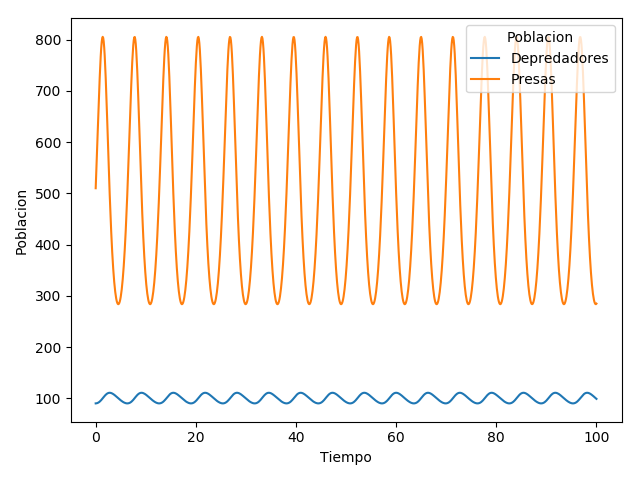
\includegraphics[scale=0.4]{img/2-90-510.png}
	  \caption{x=90,  y=510}
	\end{minipage}%
	\begin{minipage}{0.5\textwidth}
	  \centering
	  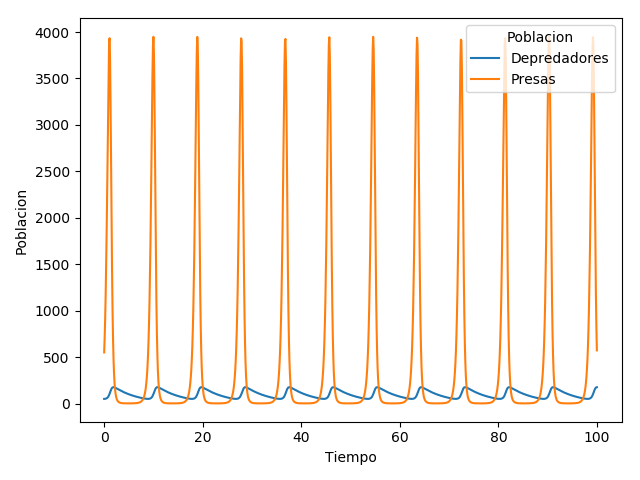
\includegraphics[scale=0.4]{img/2-50-550.png}
	  \caption{x=50,  y=550}
	\end{minipage}
\end{figure}

En estos casos, podemos ver cómo las poblaciones van oscilando e intentando mantener un equilibrio. El número de depredadores no puede crecer
sin presas, mientras que el de presas no dejará de crecer. Sin embargo, cuando un valor está cerca del otro, disminuirá el número de presas
ante el crecimiento de los depredadores, ya que las primeras son el alimento de los segundos.

También podemos ver cómo aumentar o disminuir la cantidad de presas no influye tanto como aumentar o disminuir la cantidad de depredadores.
Si nos fijamos en las figuras 3 y 4, son prácticamente iguales, ya que la única diferencia entre ellas han sido 10 presas; mientras que entre
las gráficas 2 y 4, con una diferencia de 10 depredadores, vemos que son completamente distintas.

Por otro parte, si nos fijamos en la última gráfica, vemos que no hay una clara oscilación. Esto se debe a los valores iniciales que les
hemos dado están muy alejados unos de otros y que llegue un punto en el que no haya interacción presa-depredador. Cuando la interacción
presa-depredador está ausente, el número de presas aumenta exponencialmente, mientras que el de zorros disminuye exponencialmente (y viceversa).
Por lo tanto, no es necesario considerar la presencia de oscilación.

 En nuestro caso, como el número de presas al principio es bastante alto, aumenta exponencialmente, lo que provoca un aumento gradual en el
 número de depredadores. Como resultado, se produce una rápida disminución en el número de presas y una disminución exponencial en el número
 de depredadores.


 \section{Comparación en el plano x-y}

 En el apartado anterior hemos comparado la población de ambas especies en función del tiempo, y obteniendo así una gráfica con las líneas
 correspondientes a cada una de ellas. Pero, ¿y si las visualizamos la evolución en una representación gráfica de los valores de $x$ frente
 a los de $y$, es decir, en el plano \textit{x-y}?

 Para ello vamos a utilizar el mismo $script$ utilizado anteriormente, pero esta vez cambiando los datos a mostrar. A continuación, mostramos
 el resultado de las mismas ejecuciones anteriores e intentaremos sacar alguna conclusión a partir de ellas.
 \begin{figure}[H]
	\centering
	\begin{minipage}{0.5\textwidth}
	  \centering
	  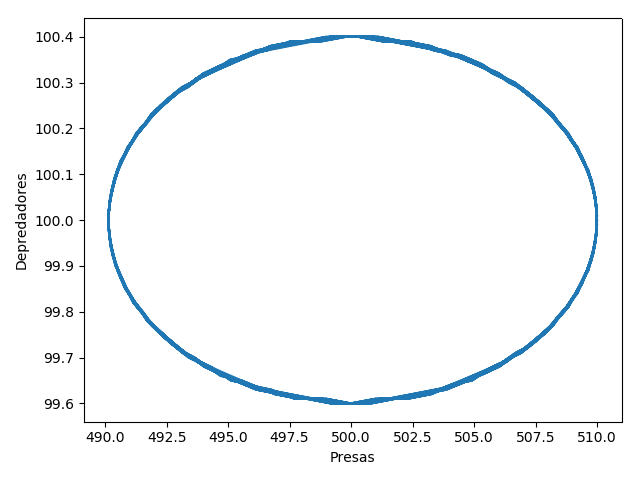
\includegraphics[scale=0.37]{img/3-100-510.png}
	  \caption{x=100,  y=510}
	\end{minipage}%
	\begin{minipage}{0.5\textwidth}
	  \centering
	  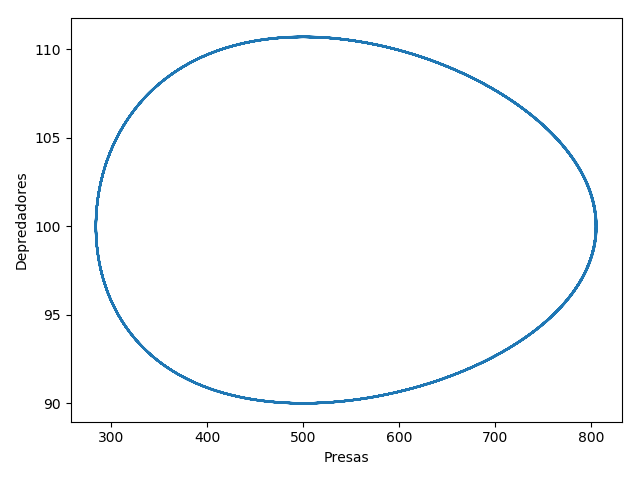
\includegraphics[scale=0.37]{img/3-90-500.png}
	  \caption{x=90,  y=500}
	\end{minipage}
\end{figure}

\begin{figure}[H]
	\centering
	\begin{minipage}{0.5\textwidth}
	  \centering
	  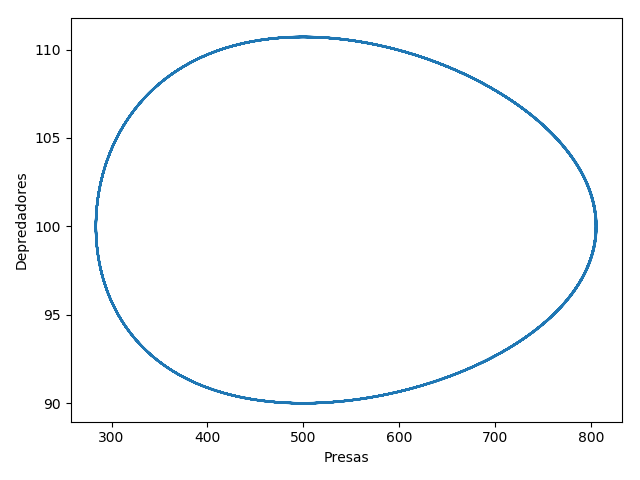
\includegraphics[scale=0.4]{img/3-90-510.png}
	  \caption{x=90,  y=510}
	\end{minipage}%
	\begin{minipage}{0.5\textwidth}
	  \centering
	  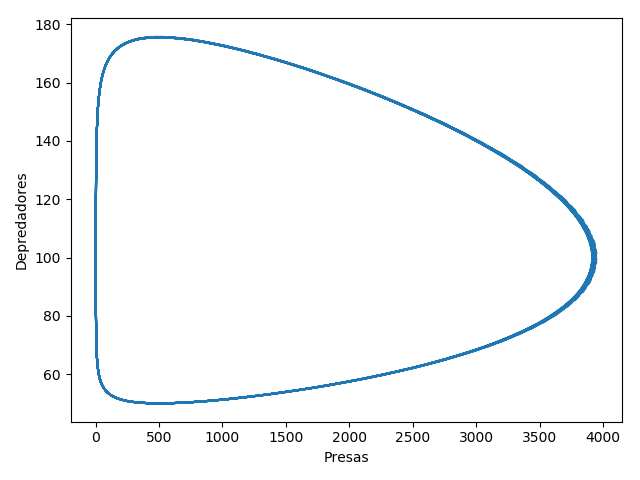
\includegraphics[scale=0.4]{img/3-50-550.png}
	  \caption{x=50,  y=550}
	\end{minipage}
\end{figure}

Como podemos ver, para todos los casos se produce una curva cerrada. La relación implícita entre las variables viene dada por la siguiente
ecuación $V=\delta x-\gamma ln(x)+\beta y-\alpha ln(y)$, donde V es una constante que depende de las condiciones iniciales y se conserva en
cada curva.

En cuanto a la diferencia entre las curvas con unos valores iniciales y otros, podemos ver cómo, a medida que distanciamos los valores, la
curva deja de ser tan circular y pasa a ser más irregular.

También podemos observar que en cada ciclo, la población de presas se reduce a números extremadamente bajos, mientras que la población de
depredadores sigue siendo considerable hasta en su nivel más bajo. En condiciones reales, esta variabilidad en la población junto con factores
externos o el ciclo de vida de las presas, podría hacer que la especie se extinga, y en consecuencia, también los depredadores (si esta es
su principal o única fuente de alimento).



\section{Experimentación cambiando las constantes $a_{ij}$}

En este apartado vamos a cambiar uno a uno estos valores para ver cómo afectan al modelo. Estudiaremos varios gráficos, pero vamos a comenzar
con una población inicial de 100 depredadores y de 500 presas, ya que es el modelo en equilibrio y donde más se van a notar los cambios. Vamos
a incrementar el valor de $a_{12}$, el cual representa que los depredadores son cazadores más eficientes (capturan más presas), pasándolo de
0.05 a 0.075. Este ha sido el resultado:
\begin{figure}[H]
	\centering
	\begin{minipage}{0.5\textwidth}
		\centering
		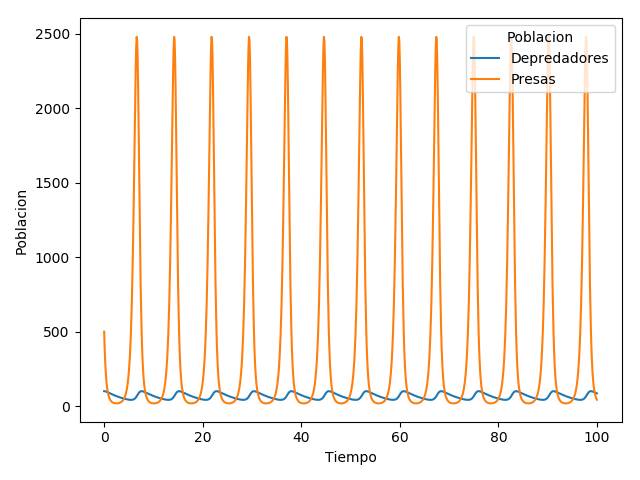
\includegraphics[scale=0.4]{img/4-a12-100-500.png}
		\caption{x=100, y=500, $a_{12}$=0.075}
	\end{minipage}%
	\begin{minipage}{0.5\textwidth}
		\centering
		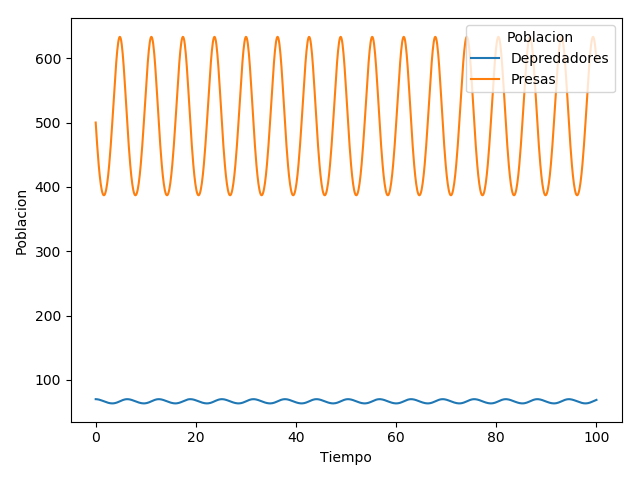
\includegraphics[scale=0.4]{img/4-a12-70-500.png}
		\caption{x=70, y=500, $a_{12}$=0.075}
	\end{minipage}
\end{figure}

Como podemos ver, un aumento de un 50\% de eficiencia a la hora de cazar hace que el modelo se desestabilice bastante, llegando casi a perder
por completo la oscilación (la interacción presa-depredador). En la imagen de la derecha podemos ver cómo, con unos depredadores eficientes,
podemos compensar una falta de estos en la población inicial, manteniendo el sistema bastante equilibrado.

Ahora vamos a incrementar el valor de $a_{11}$, el cual indica que las presas tienen una tasa de crecimiento más rápida, pasándolo de 5 crías
por pareja a 6. Este ha sido el resultado:
\begin{figure}[H]
	\centering
	\begin{minipage}{0.5\textwidth}
		\centering
		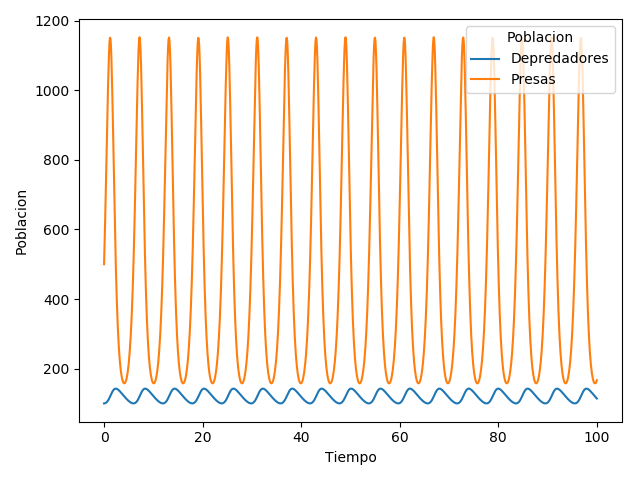
\includegraphics[scale=0.4]{img/4-a11-100-500.png}
		\caption{x=100, y=500, $a_{11}$=6}
	\end{minipage}%
	\begin{minipage}{0.5\textwidth}
		\centering
		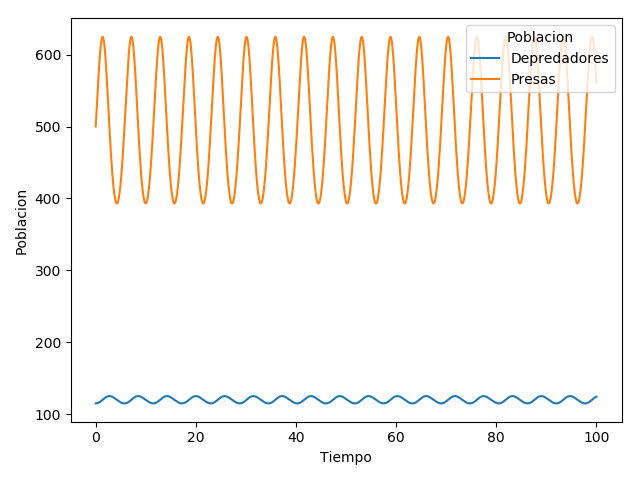
\includegraphics[scale=0.4]{img/4-a11-115-500.png}
		\caption{x=115, y=500, $a_{11}$=6}
	\end{minipage}
\end{figure}

Como podemos ver, tenemos una situación muy similar a la anterior, ya que también desestabilizamos bastante el modelo. No obstante, en este caso
ha sido al contrario, ya que estamos aumentando el número de conejos al año. En la imagen de la derecha podemos ver cómo mantenemos el sistema
más o menos equilibrado, pero aumentando el número de depredadores inicial, en vez de reducirlo.

A continuación, vamos a probar con el parámetro $a_{22}$, el cual representa la longevidad de los depredadores.


\end{document}



